% REV00 Tue 04 May 2021 13:55:16 WIB
% START Tue 04 May 2021 13:55:16 WIB

\chapter{XXX}

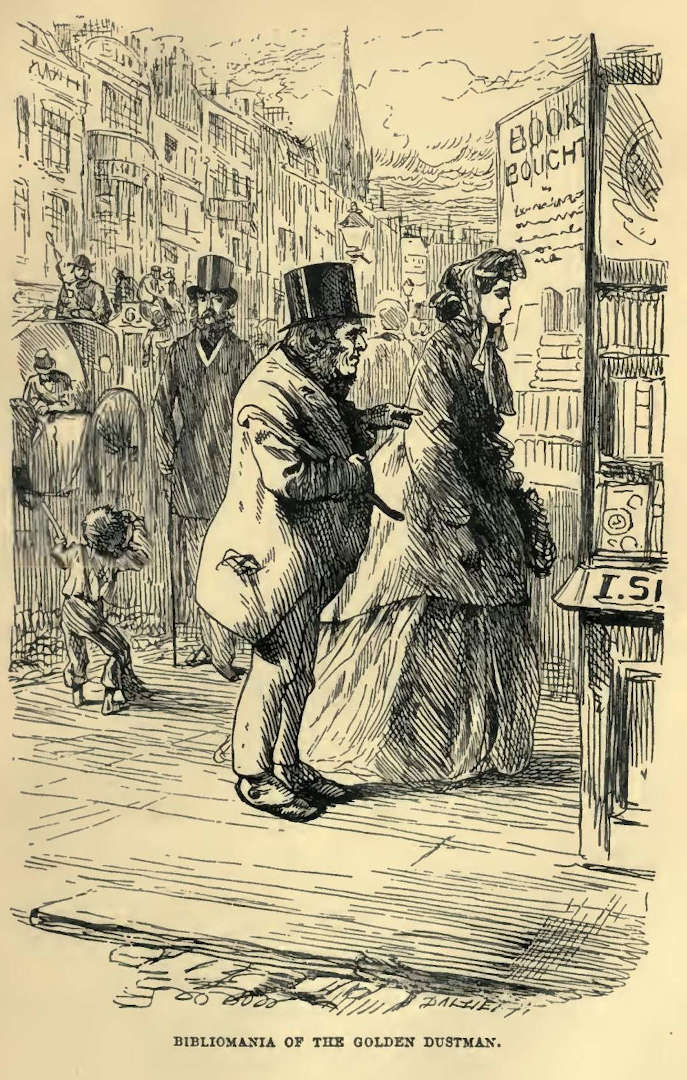
\includegraphics[scale=2.3]{03-05-01}

Chapter 16

PERSONS AND THINGS IN GENERAL


Mr and Mrs John Harmon’s first delightful occupation was, to set all
matters right that had strayed in any way wrong, or that might, could,
would, or should, have strayed in any way wrong, while their name was in
abeyance. In tracing out affairs for which John’s fictitious death was
to be considered in any way responsible, they used a very broad and free
construction; regarding, for instance, the dolls’ dressmaker as having
a claim on their protection, because of her association with Mrs Eugene
Wrayburn, and because of Mrs Eugene’s old association, in her turn, with
the dark side of the story. It followed that the old man, Riah, as a
good and serviceable friend to both, was not to be disclaimed. Nor even
Mr Inspector, as having been trepanned into an industrious hunt on a
false scent. It may be remarked, in connexion with that worthy officer,
that a rumour shortly afterwards pervaded the Force, to the effect that
he had confided to Miss Abbey Potterson, over a jug of mellow flip in
the bar of the Six Jolly Fellowship Porters, that he ‘didn’t stand to
lose a farthing’ through Mr Harmon’s coming to life, but was quite as
well satisfied as if that gentleman had been barbarously murdered, and
he (Mr Inspector) had pocketed the government reward.

In all their arrangements of such nature, Mr and Mrs John Harmon derived
much assistance from their eminent solicitor, Mr Mortimer Lightwood; who
laid about him professionally with such unwonted despatch and intention,
that a piece of work was vigorously pursued as soon as cut out; whereby
Young Blight was acted on as by that transatlantic dram which is
poetically named An Eye-Opener, and found himself staring at real
clients instead of out of window. The accessibility of Riah proving
very useful as to a few hints towards the disentanglement of Eugene’s
affairs, Lightwood applied himself with infinite zest to attacking and
harassing Mr Fledgeby: who, discovering himself in danger of being blown
into the air by certain explosive transactions in which he had been
engaged, and having been sufficiently flayed under his beating, came
to a parley and asked for quarter. The harmless Twemlow profited by
the conditions entered into, though he little thought it. Mr Riah
unaccountably melted; waited in person on him over the stable yard in
Duke Street, St James’s, no longer ravening but mild, to inform him
that payment of interest as heretofore, but henceforth at Mr Lightwood’s
offices, would appease his Jewish rancour; and departed with the secret
that Mr John Harmon had advanced the money and become the creditor.
Thus, was the sublime Snigsworth’s wrath averted, and thus did he snort
no larger amount of moral grandeur at the Corinthian column in the
print over the fireplace, than was normally in his (and the British)
constitution.


Mrs Wilfer’s first visit to the Mendicant’s bride at the new abode of
Mendicancy, was a grand event. Pa had been sent for into the City,
on the very day of taking possession, and had been stunned with
astonishment, and brought-to, and led about the house by one ear, to
behold its various treasures, and had been enraptured and enchanted. Pa
had also been appointed Secretary, and had been enjoined to give instant
notice of resignation to Chicksey, Veneering, and Stobbles, for ever and
ever. But Ma came later, and came, as was her due, in state.

The carriage was sent for Ma, who entered it with a bearing worthy of
the occasion, accompanied, rather than supported, by Miss Lavinia, who
altogether declined to recognize the maternal majesty. Mr George Sampson
meekly followed. He was received in the vehicle, by Mrs Wilfer, as if
admitted to the honour of assisting at a funeral in the family, and she
then issued the order, ‘Onward!’ to the Mendicant’s menial.

‘I wish to goodness, Ma,’ said Lavvy, throwing herself back among the
cushions, with her arms crossed, ‘that you’d loll a little.’

‘How!’ repeated Mrs Wilfer. ‘Loll!’

‘Yes, Ma.’

‘I hope,’ said the impressive lady, ‘I am incapable of it.’

‘I am sure you look so, Ma. But why one should go out to dine with one’s
own daughter or sister, as if one’s under-petticoat was a backboard, I
do NOT understand.’

‘Neither do I understand,’ retorted Mrs Wilfer, with deep scorn, ‘how
a young lady can mention the garment in the name of which you have
indulged. I blush for you.’

‘Thank you, Ma,’ said Lavvy, yawning, ‘but I can do it for myself, I am
obliged to you, when there’s any occasion.’

Here, Mr Sampson, with the view of establishing harmony, which he never
under any circumstances succeeded in doing, said with an agreeable
smile: ‘After all, you know, ma’am, we know it’s there.’ And immediately
felt that he had committed himself.

‘We know it’s there!’ said Mrs Wilfer, glaring.

‘Really, George,’ remonstrated Miss Lavinia, ‘I must say that I don’t
understand your allusions, and that I think you might be more delicate
and less personal.’

‘Go it!’ cried Mr Sampson, becoming, on the shortest notice, a prey to
despair. ‘Oh yes! Go it, Miss Lavinia Wilfer!’

‘What you may mean, George Sampson, by your omnibus-driving expressions,
I cannot pretend to imagine. Neither,’ said Miss Lavinia, ‘Mr George
Sampson, do I wish to imagine. It is enough for me to know in my own
heart that I am not going to--’ having imprudently got into a sentence
without providing a way out of it, Miss Lavinia was constrained to
close with ‘going to it’. A weak conclusion which, however, derived some
appearance of strength from disdain.

‘Oh yes!’ cried Mr Sampson, with bitterness. ‘Thus it ever is. I
never--’

‘If you mean to say,’ Miss Lavvy cut him short, that you never brought
up a young gazelle, you may save yourself the trouble, because nobody
in this carriage supposes that you ever did. We know you better.’ (As if
this were a home-thrust.)

‘Lavinia,’ returned Mr Sampson, in a dismal vein, ‘I did not mean to
say so. What I did mean to say, was, that I never expected to retain my
favoured place in this family, after Fortune shed her beams upon it. Why
do you take me,’ said Mr Sampson, ‘to the glittering halls with which
I can never compete, and then taunt me with my moderate salary? Is it
generous? Is it kind?’

The stately lady, Mrs Wilfer, perceiving her opportunity of delivering a
few remarks from the throne, here took up the altercation.

‘Mr Sampson,’ she began, ‘I cannot permit you to misrepresent the
intentions of a child of mine.’

‘Let him alone, Ma,’ Miss Lavvy interposed with haughtiness. ‘It is
indifferent to me what he says or does.’

‘Nay, Lavinia,’ quoth Mrs Wilfer, ‘this touches the blood of the family.
If Mr George Sampson attributes, even to my youngest daughter--’

[‘I don’t see why you should use the word “even”, Ma,’ Miss Lavvy
interposed, ‘because I am quite as important as any of the others.’)

‘Peace!’ said Mrs Wilfer, solemnly. ‘I repeat, if Mr George Sampson
attributes, to my youngest daughter, grovelling motives, he attributes
them equally to the mother of my youngest daughter. That mother
repudiates them, and demands of Mr George Sampson, as a youth of honour,
what he WOULD have? I may be mistaken--nothing is more likely--but Mr
George Sampson,’ proceeded Mrs Wilfer, majestically waving her gloves,
‘appears to me to be seated in a first-class equipage. Mr George Sampson
appears to me to be on his way, by his own admission, to a residence
that may be termed Palatial. Mr George Sampson appears to me to be
invited to participate in the--shall I say the--Elevation which has
descended on the family with which he is ambitious, shall I say to
Mingle? Whence, then, this tone on Mr Sampson’s part?’

‘It is only, ma’am,’ Mr Sampson explained, in exceedingly low spirits,
‘because, in a pecuniary sense, I am painfully conscious of my
unworthiness. Lavinia is now highly connected. Can I hope that she will
still remain the same Lavinia as of old? And is it not pardonable if
I feel sensitive, when I see a disposition on her part to take me up
short?’

‘If you are not satisfied with your position, sir,’ observed Miss
Lavinia, with much politeness, ‘we can set you down at any turning you
may please to indicate to my sister’s coachman.’

‘Dearest Lavinia,’ urged Mr Sampson, pathetically, ‘I adore you.’

‘Then if you can’t do it in a more agreeable manner,’ returned the young
lady, ‘I wish you wouldn’t.’

‘I also,’ pursued Mr Sampson, ‘respect you, ma’am, to an extent which
must ever be below your merits, I am well aware, but still up to an
uncommon mark. Bear with a wretch, Lavinia, bear with a wretch, ma’am,
who feels the noble sacrifices you make for him, but is goaded almost to
madness,’ Mr Sampson slapped his forehead, ‘when he thinks of competing
with the rich and influential.’

‘When you have to compete with the rich and influential, it will
probably be mentioned to you,’ said Miss Lavvy, ‘in good time. At least,
it will if the case is MY case.’

Mr Sampson immediately expressed his fervent Opinion that this was ‘more
than human’, and was brought upon his knees at Miss Lavinia’s feet.

It was the crowning addition indispensable to the full enjoyment of both
mother and daughter, to bear Mr Sampson, a grateful captive, into the
glittering halls he had mentioned, and to parade him through the same,
at once a living witness of their glory, and a bright instance of their
condescension. Ascending the staircase, Miss Lavinia permitted him to
walk at her side, with the air of saying: ‘Notwithstanding all these
surroundings, I am yours as yet, George. How long it may last is another
question, but I am yours as yet.’ She also benignantly intimated to him,
aloud, the nature of the objects upon which he looked, and to which he
was unaccustomed: as, ‘Exotics, George,’ ‘An aviary, George,’ ‘An
ormolu clock, George,’ and the like. While, through the whole of the
decorations, Mrs Wilfer led the way with the bearing of a Savage Chief,
who would feel himself compromised by manifesting the slightest token of
surprise or admiration.

Indeed, the bearing of this impressive woman, throughout the day, was a
pattern to all impressive women under similar circumstances. She renewed
the acquaintance of Mr and Mrs Boffin, as if Mr and Mrs Boffin had said
of her what she had said of them, and as if Time alone could quite wear
her injury out. She regarded every servant who approached her, as her
sworn enemy, expressly intending to offer her affronts with the dishes,
and to pour forth outrages on her moral feelings from the decanters.
She sat erect at table, on the right hand of her son-in-law, as half
suspecting poison in the viands, and as bearing up with native force of
character against other deadly ambushes. Her carriage towards Bella was
as a carriage towards a young lady of good position, whom she had met in
society a few years ago. Even when, slightly thawing under the influence
of sparkling champagne, she related to her son-in-law some passages of
domestic interest concerning her papa, she infused into the narrative
such Arctic suggestions of her having been an unappreciated blessing to
mankind, since her papa’s days, and also of that gentleman’s having
been a frosty impersonation of a frosty race, as struck cold to the
very soles of the feet of the hearers. The Inexhaustible being produced,
staring, and evidently intending a weak and washy smile shortly, no
sooner beheld her, than it was stricken spasmodic and inconsolable. When
she took her leave at last, it would have been hard to say whether it
was with the air of going to the scaffold herself, or of leaving the
inmates of the house for immediate execution. Yet, John Harmon enjoyed
it all merrily, and told his wife, when he and she were alone, that her
natural ways had never seemed so dearly natural as beside this foil,
and that although he did not dispute her being her father’s daughter,
he should ever remain stedfast in the faith that she could not be her
mother’s.


This visit was, as has been said, a grand event. Another event, not
grand but deemed in the house a special one, occurred at about the same
period; and this was, the first interview between Mr Sloppy and Miss
Wren.

The dolls’ dressmaker, being at work for the Inexhaustible upon a
full-dressed doll some two sizes larger than that young person, Mr
Sloppy undertook to call for it, and did so.

‘Come in, sir,’ said Miss Wren, who was working at her bench. ‘And who
may you be?’

Mr Sloppy introduced himself by name and buttons.

‘Oh indeed!’ cried Jenny. ‘Ah! I have been looking forward to knowing
you. I heard of your distinguishing yourself.’

‘Did you, Miss?’ grinned Sloppy. ‘I am sure I am glad to hear it, but I
don’t know how.’

‘Pitching somebody into a mud-cart,’ said Miss Wren.

‘Oh! That way!’ cried Sloppy. ‘Yes, Miss.’ And threw back his head and
laughed.

‘Bless us!’ exclaimed Miss Wren, with a start. ‘Don’t open your mouth
as wide as that, young man, or it’ll catch so, and not shut again some
day.’

Mr Sloppy opened it, if possible, wider, and kept it open until his
laugh was out.

‘Why, you’re like the giant,’ said Miss Wren, ‘when he came home in the
land of Beanstalk, and wanted Jack for supper.’

‘Was he good-looking, Miss?’ asked Sloppy.

‘No,’ said Miss Wren. ‘Ugly.’

Her visitor glanced round the room--which had many comforts in it now,
that had not been in it before--and said: ‘This is a pretty place,
Miss.’

‘Glad you think so, sir,’ returned Miss Wren. ‘And what do you think of
Me?’

The honesty of Mr Sloppy being severely taxed by the question, he
twisted a button, grinned, and faltered.

‘Out with it!’ said Miss Wren, with an arch look. ‘Don’t you think me
a queer little comicality?’ In shaking her head at him after asking the
question, she shook her hair down.

‘Oh!’ cried Sloppy, in a burst of admiration. ‘What a lot, and what a
colour!’

Miss Wren, with her usual expressive hitch, went on with her work. But,
left her hair as it was; not displeased by the effect it had made.

‘You don’t live here alone; do you, Miss?’ asked Sloppy.

‘No,’ said Miss Wren, with a chop. ‘Live here with my fairy godmother.’

‘With;’ Mr Sloppy couldn’t make it out; ‘with who did you say, Miss?’

‘Well!’ replied Miss Wren, more seriously. ‘With my second father. Or
with my first, for that matter.’ And she shook her head, and drew a
sigh. ‘If you had known a poor child I used to have here,’ she added,
‘you’d have understood me. But you didn’t, and you can’t. All the
better!’

‘You must have been taught a long time,’ said Sloppy, glancing at the
array of dolls in hand, ‘before you came to work so neatly, Miss, and
with such a pretty taste.’

‘Never was taught a stitch, young man!’ returned the dress-maker,
tossing her head. ‘Just gobbled and gobbled, till I found out how to do
it. Badly enough at first, but better now.’

‘And here have I,’ said Sloppy, in something of a self-reproachful tone,
‘been a learning and a learning, and here has Mr Boffin been a paying
and a paying, ever so long!’

‘I have heard what your trade is,’ observed Miss Wren; ‘it’s
cabinet-making.’

Mr Sloppy nodded. ‘Now that the Mounds is done with, it is. I’ll tell
you what, Miss. I should like to make you something.’

‘Much obliged. But what?’

‘I could make you,’ said Sloppy, surveying the room, ‘I could make you
a handy set of nests to lay the dolls in. Or I could make you a handy
little set of drawers, to keep your silks and threads and scraps in. Or
I could turn you a rare handle for that crutch-stick, if it belongs to
him you call your father.’

‘It belongs to me,’ returned the little creature, with a quick flush of
her face and neck. ‘I am lame.’

Poor Sloppy flushed too, for there was an instinctive delicacy behind
his buttons, and his own hand had struck it. He said, perhaps, the best
thing in the way of amends that could be said. ‘I am very glad it’s
yours, because I’d rather ornament it for you than for any one else.
Please may I look at it?’

Miss Wren was in the act of handing it to him over her bench, when she
paused. ‘But you had better see me use it,’ she said, sharply. ‘This is
the way. Hoppetty, Kicketty, Pep-peg-peg. Not pretty; is it?’

‘It seems to me that you hardly want it at all,’ said Sloppy.

The little dressmaker sat down again, and gave it into his hand, saying,
with that better look upon her, and with a smile: ‘Thank you!’

‘And as concerning the nests and the drawers,’ said Sloppy, after
measuring the handle on his sleeve, and softly standing the stick aside
against the wall, ‘why, it would be a real pleasure to me. I’ve heerd
tell that you can sing most beautiful; and I should be better paid with
a song than with any money, for I always loved the likes of that, and
often giv’ Mrs Higden and Johnny a comic song myself, with “Spoken” in
it. Though that’s not your sort, I’ll wager.’

‘You are a very kind young man,’ returned the dressmaker; ‘a really kind
young man. I accept your offer.--I suppose He won’t mind,’ she added as
an afterthought, shrugging her shoulders; ‘and if he does, he may!’

‘Meaning him that you call your father, Miss,’ asked Sloppy.

‘No, no,’ replied Miss Wren. ‘Him, Him, Him!’

‘Him, him, him?’ repeated Sloppy; staring about, as if for Him.

‘Him who is coming to court and marry me,’ returned Miss Wren. ‘Dear me,
how slow you are!’

‘Oh! HIM!’ said Sloppy. And seemed to turn thoughtful and a little
troubled. ‘I never thought of him. When is he coming, Miss?’

‘What a question!’ cried Miss Wren. ‘How should I know!’

‘Where is he coming from, Miss?’

‘Why, good gracious, how can I tell! He is coming from somewhere or
other, I suppose, and he is coming some day or other, I suppose. I don’t
know any more about him, at present.’

This tickled Mr Sloppy as an extraordinarily good joke, and he threw
back his head and laughed with measureless enjoyment. At the sight of
him laughing in that absurd way, the dolls’ dressmaker laughed very
heartily indeed. So they both laughed, till they were tired.

‘There, there, there!’ said Miss Wren. ‘For goodness’ sake, stop, Giant,
or I shall be swallowed up alive, before I know it. And to this minute
you haven’t said what you’ve come for.’

‘I have come for little Miss Harmonses doll,’ said Sloppy.

‘I thought as much,’ remarked Miss Wren, ‘and here is little Miss
Harmonses doll waiting for you. She’s folded up in silver paper, you
see, as if she was wrapped from head to foot in new Bank notes. Take
care of her, and there’s my hand, and thank you again.’

‘I’ll take more care of her than if she was a gold image,’ said Sloppy,
‘and there’s both MY hands, Miss, and I’ll soon come back again.’


But, the greatest event of all, in the new life of Mr and Mrs John
Harmon, was a visit from Mr and Mrs Eugene Wrayburn. Sadly wan and worn
was the once gallant Eugene, and walked resting on his wife’s arm, and
leaning heavily upon a stick. But, he was daily growing stronger and
better, and it was declared by the medical attendants that he might not
be much disfigured by-and-by. It was a grand event, indeed, when Mr
and Mrs Eugene Wrayburn came to stay at Mr and Mrs John Harmon’s house:
where, by the way, Mr and Mrs Boffin (exquisitely happy, and daily
cruising about, to look at shops,) were likewise staying indefinitely.

To Mr Eugene Wrayburn, in confidence, did Mrs John Harmon impart what
she had known of the state of his wife’s affections, in his reckless
time. And to Mrs John Harmon, in confidence, did Mr Eugene Wrayburn
impart that, please God, she should see how his wife had changed him!

‘I make no protestations,’ said Eugene; ‘--who does, who means them!--I
have made a resolution.’

‘But would you believe, Bella,’ interposed his wife, coming to resume
her nurse’s place at his side, for he never got on well without her:
‘that on our wedding day he told me he almost thought the best thing he
could do, was to die?’

‘As I didn’t do it, Lizzie,’ said Eugene, ‘I’ll do that better thing you
suggested--for your sake.’

That same afternoon, Eugene lying on his couch in his own room upstairs,
Lightwood came to chat with him, while Bella took his wife out for a
ride. ‘Nothing short of force will make her go,’ Eugene had said; so,
Bella had playfully forced her.

‘Dear old fellow,’ Eugene began with Lightwood, reaching up his hand,
‘you couldn’t have come at a better time, for my mind is full, and I
want to empty it. First, of my present, before I touch upon my future.
M. R. F., who is a much younger cavalier than I, and a professed admirer
of beauty, was so affable as to remark the other day (he paid us a visit
of two days up the river there, and much objected to the accommodation
of the hotel), that Lizzie ought to have her portrait painted. Which,
coming from M. R. F., may be considered equivalent to a melodramatic
blessing.’

‘You are getting well,’ said Mortimer, with a smile.

‘Really,’ said Eugene, ‘I mean it. When M. R. F. said that, and followed
it up by rolling the claret (for which he called, and I paid), in his
mouth, and saying, “My dear son, why do you drink this trash?” it was
tantamount in him--to a paternal benediction on our union, accompanied
with a gush of tears. The coolness of M. R. F. is not to be measured by
ordinary standards.’

‘True enough,’ said Lightwood.

‘That’s all,’ pursued Eugene, ‘that I shall ever hear from M. R. F. on
the subject, and he will continue to saunter through the world with
his hat on one side. My marriage being thus solemnly recognized at the
family altar, I have no further trouble on that score. Next, you really
have done wonders for me, Mortimer, in easing my money-perplexities, and
with such a guardian and steward beside me, as the preserver of my life
(I am hardly strong yet, you see, for I am not man enough to refer
to her without a trembling voice--she is so inexpressibly dear to me,
Mortimer!), the little that I can call my own will be more than it ever
has been. It need be more, for you know what it always has been in my
hands. Nothing.’

‘Worse than nothing, I fancy, Eugene. My own small income (I devoutly
wish that my grandfather had left it to the Ocean rather than to me!)
has been an effective Something, in the way of preventing me from
turning to at Anything. And I think yours has been much the same.’

‘There spake the voice of wisdom,’ said Eugene. ‘We are shepherds both.
In turning to at last, we turn to in earnest. Let us say no more of
that, for a few years to come. Now, I have had an idea, Mortimer, of
taking myself and my wife to one of the colonies, and working at my
vocation there.’

‘I should be lost without you, Eugene; but you may be right.’

‘No,’ said Eugene, emphatically. ‘Not right. Wrong!’

He said it with such a lively--almost angry--flash, that Mortimer showed
himself greatly surprised.

‘You think this thumped head of mine is excited?’ Eugene went on, with a
high look; ‘not so, believe me. I can say to you of the healthful music
of my pulse what Hamlet said of his. My blood is up, but wholesomely up,
when I think of it. Tell me! Shall I turn coward to Lizzie, and sneak
away with her, as if I were ashamed of her! Where would your friend’s
part in this world be, Mortimer, if she had turned coward to him, and on
immeasurably better occasion?’

‘Honourable and stanch,’ said Lightwood. ‘And yet, Eugene--’

‘And yet what, Mortimer?’

‘And yet, are you sure that you might not feel (for her sake, I say for
her sake) any slight coldness towards her on the part of--Society?’

‘O! You and I may well stumble at the word,’ returned Eugene, laughing.
‘Do we mean our Tippins?’

‘Perhaps we do,’ said Mortimer, laughing also.

‘Faith, we DO!’ returned Eugene, with great animation. ‘We may hide
behind the bush and beat about it, but we DO! Now, my wife is something
nearer to my heart, Mortimer, than Tippins is, and I owe her a little
more than I owe to Tippins, and I am rather prouder of her than I ever
was of Tippins. Therefore, I will fight it out to the last gasp, with
her and for her, here, in the open field. When I hide her, or strike
for her, faint-heartedly, in a hole or a corner, do you whom I love next
best upon earth, tell me what I shall most righteously deserve to be
told:--that she would have done well to turn me over with her foot that
night when I lay bleeding to death, and spat in my dastard face.’

The glow that shone upon him as he spoke the words, so irradiated his
features that he looked, for the time, as though he had never been
mutilated. His friend responded as Eugene would have had him respond,
and they discoursed of the future until Lizzie came back. After resuming
her place at his side, and tenderly touching his hands and his head, she
said:

‘Eugene, dear, you made me go out, but I ought to have stayed with you.
You are more flushed than you have been for many days. What have you
been doing?’

‘Nothing,’ replied Eugene, ‘but looking forward to your coming back.’

‘And talking to Mr Lightwood,’ said Lizzie, turning to him with a smile.
‘But it cannot have been Society that disturbed you.’

‘Faith, my dear love!’ retorted Eugene, in his old airy manner, as he
laughed and kissed her, ‘I rather think it WAS Society though!’

The word ran so much in Mortimer Lightwood’s thoughts as he went home to
the Temple that night, that he resolved to take a look at Society, which
he had not seen for a considerable period.



